


\tikzset{every picture/.style={line width=0.75pt}} %set default line width to 0.75pt        

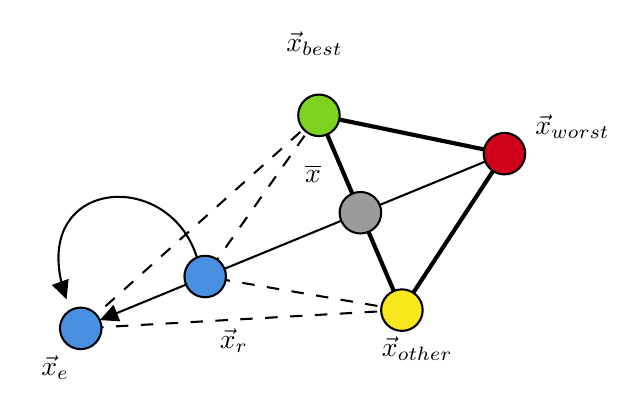
\begin{tikzpicture}[x=0.75pt,y=0.75pt,yscale=-1,xscale=1]
%uncomment if require: \path (0,914); %set diagram left start at 0, and has height of 914

%Straight Lines [id:da11343228301624042] 
\draw [line width=1.5]    (431.21,289.73) -- (520.59,308.19) ;
%Straight Lines [id:da5343513078972191] 
\draw [line width=1.5]    (471.18,383.58) -- (431.21,289.73) ;
%Straight Lines [id:da35681996429433105] 
\draw [line width=1.5]    (471.18,383.58) -- (520.59,308.19) ;
%Straight Lines [id:da35098952534036765] 
\draw    (520.59,308.19) -- (328.38,387.25) ;
\draw [shift={(325.61,388.39)}, rotate = 337.64] [fill={rgb, 255:red, 0; green, 0; blue, 0 }  ][line width=0.08]  [draw opacity=0] (8.93,-4.29) -- (0,0) -- (8.93,4.29) -- cycle    ;
%Shape: Circle [id:dp9759552457158815] 
\draw  [fill={rgb, 255:red, 155; green, 155; blue, 155 }  ,fill opacity=1 ] (441.99,340.57) .. controls (439.83,335.49) and (442.2,329.62) .. (447.28,327.45) .. controls (452.36,325.29) and (458.23,327.65) .. (460.4,332.74) .. controls (462.56,337.82) and (460.19,343.69) .. (455.11,345.85) .. controls (450.03,348.02) and (444.16,345.65) .. (441.99,340.57) -- cycle ;
%Shape: Circle [id:dp25947223717017986] 
\draw  [fill={rgb, 255:red, 208; green, 2; blue, 27 }  ,fill opacity=1 ] (511.39,312.1) .. controls (509.22,307.02) and (511.59,301.15) .. (516.67,298.99) .. controls (521.75,296.82) and (527.62,299.19) .. (529.79,304.27) .. controls (531.95,309.35) and (529.59,315.22) .. (524.51,317.39) .. controls (519.43,319.55) and (513.55,317.19) .. (511.39,312.1) -- cycle ;
%Straight Lines [id:da5926907267680663] 
\draw  [dash pattern={on 4.5pt off 4.5pt}]  (471.18,383.58) -- (376.4,367.39) ;
%Straight Lines [id:da13882970361087188] 
\draw  [dash pattern={on 4.5pt off 4.5pt}]  (431.21,289.73) -- (376.4,367.39) ;
%Shape: Circle [id:dp08877809464082187] 
\draw  [fill={rgb, 255:red, 74; green, 144; blue, 226 }  ,fill opacity=1 ] (385.58,363.41) .. controls (387.77,368.47) and (385.45,374.36) .. (380.38,376.56) .. controls (375.32,378.76) and (369.43,376.43) .. (367.23,371.37) .. controls (365.03,366.3) and (367.36,360.41) .. (372.42,358.21) .. controls (377.49,356.01) and (383.38,358.34) .. (385.58,363.41) -- cycle ;
%Straight Lines [id:da6283525001318553] 
\draw  [dash pattern={on 4.5pt off 4.5pt}]  (471.18,383.58) -- (316.43,392.37) ;
%Straight Lines [id:da46426000871766093] 
\draw  [dash pattern={on 4.5pt off 4.5pt}]  (431.21,289.73) -- (316.43,392.37) ;
%Shape: Circle [id:dp39491065736136166] 
\draw  [fill={rgb, 255:red, 74; green, 144; blue, 226 }  ,fill opacity=1 ] (325.61,388.39) .. controls (327.81,393.46) and (325.48,399.35) .. (320.41,401.54) .. controls (315.35,403.74) and (309.46,401.42) .. (307.26,396.35) .. controls (305.06,391.28) and (307.39,385.39) .. (312.46,383.2) .. controls (317.52,381) and (323.41,383.32) .. (325.61,388.39) -- cycle ;
%Shape: Circle [id:dp8580698815752372] 
\draw  [fill={rgb, 255:red, 248; green, 231; blue, 28 }  ,fill opacity=1 ] (461.98,387.49) .. controls (459.82,382.41) and (462.18,376.54) .. (467.26,374.38) .. controls (472.34,372.21) and (478.22,374.58) .. (480.38,379.66) .. controls (482.54,384.74) and (480.18,390.61) .. (475.1,392.78) .. controls (470.02,394.94) and (464.14,392.58) .. (461.98,387.49) -- cycle ;
%Shape: Circle [id:dp07260801254247773] 
\draw  [fill={rgb, 255:red, 126; green, 211; blue, 33 }  ,fill opacity=1 ] (422.01,293.65) .. controls (419.85,288.57) and (422.21,282.7) .. (427.29,280.53) .. controls (432.37,278.37) and (438.25,280.73) .. (440.41,285.81) .. controls (442.57,290.9) and (440.21,296.77) .. (435.13,298.93) .. controls (430.05,301.1) and (424.17,298.73) .. (422.01,293.65) -- cycle ;
%Curve Lines [id:da945800091817379] 
\draw    (308.46,374.97) .. controls (291.38,320.13) and (358.7,314.11) .. (372.42,358.21) ;
\draw [shift={(309.61,378.39)}, rotate = 250.1] [fill={rgb, 255:red, 0; green, 0; blue, 0 }  ][line width=0.08]  [draw opacity=0] (8.93,-4.29) -- (0,0) -- (8.93,4.29) -- cycle    ;

% Text Node
\draw (414,248) node [anchor=north west][inner sep=0.75pt]   [align=left] {$\displaystyle \vec{x}_{best}$};
% Text Node
\draw (534,288) node [anchor=north west][inner sep=0.75pt]   [align=left] {$\displaystyle \vec{x}_{worst}$};
% Text Node
\draw (460,395) node [anchor=north west][inner sep=0.75pt]   [align=left] {$\displaystyle \vec{x}_{other}$};
% Text Node
\draw (423,312) node [anchor=north west][inner sep=0.75pt]   [align=left] {$\displaystyle \overline{x}$};
% Text Node
\draw (382,391) node [anchor=north west][inner sep=0.75pt]   [align=left] {$\displaystyle \vec{x}_{r}$};
% Text Node
\draw (296,404) node [anchor=north west][inner sep=0.75pt]   [align=left] {$\displaystyle \vec{x}_{e}$};


\end{tikzpicture}